\newpage

\section{Dataset Description}

\quad For this project, we were provided with an excel file called "bebidas.xlsx", within which are the daily sales records of each of the two beverages made available by the company in question, within that excel file there are still other relevant data, which will be detailed afterwards. \\

In the following image we have a print of the columns of the dataset mentioned above:

\begin{figure}[H]
    \centering
    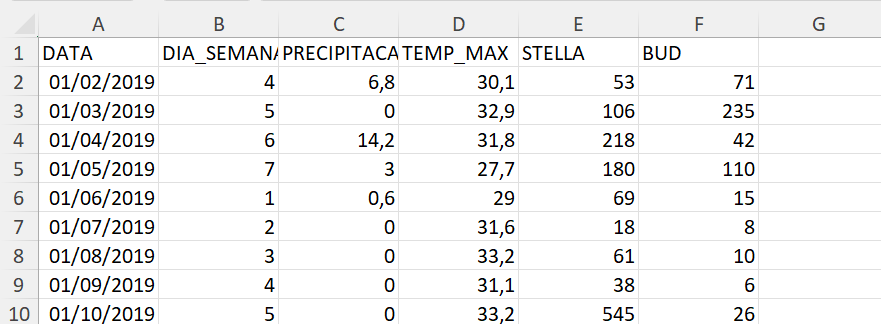
\includegraphics[width=0.8\textwidth]{assets/dataset.png}
    \caption{Project Dataset}
    \label{fig:dataset}
    \end{figure}


The following dataset is compose of 6 columns, they being:

\quad \textbullet DATA: This column represents the date the records are from;

\quad \textbullet DIA\_SEMANA: This column represents the day of the week, where 1 is Sunday, 2 is Monday, 3 is Tuesday, 4 is Wednesday, 5 is Thursday, 6 is Friday and 7 is Saturday;

\quad \textbullet PRECIPITACAO: This column represents the total of precipitation in mm in that day;

\quad \textbullet TEMP\_MAX: This column represents the daily maximum temperature in Celcius from that day;

\quad \textbullet STELLA: This column represents the number of STELLA drinks that where sold in that day;

\quad \textbullet BUD: This column represents the number of BUD drinks that where sold in that day.\\


These  two diagrams represent the sales of each of the drinks provided in the dataset:
\\
\begin{figure}[H]
    \centering
    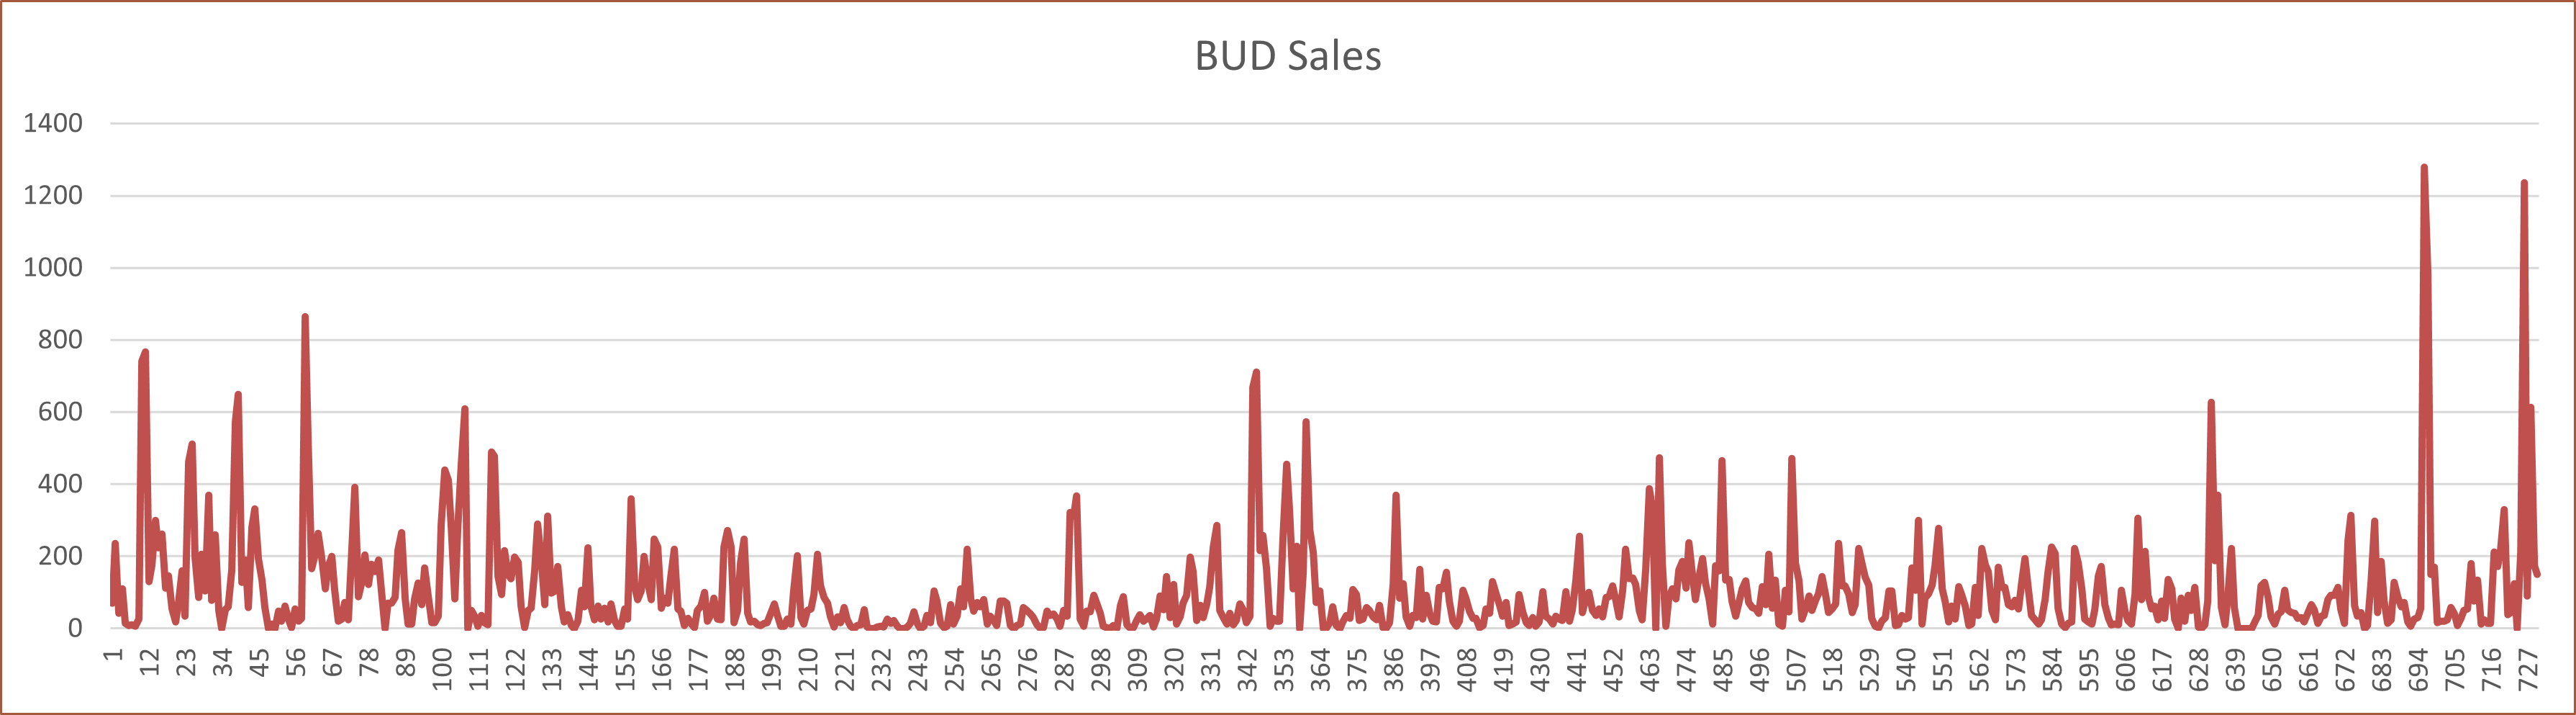
\includegraphics[width=0.8\textwidth]{assets/BUD.png}
    \caption{BUD Sales}
    \label{fig:bud_sales}
    \end{figure}

\begin{figure}[H]
    \centering
    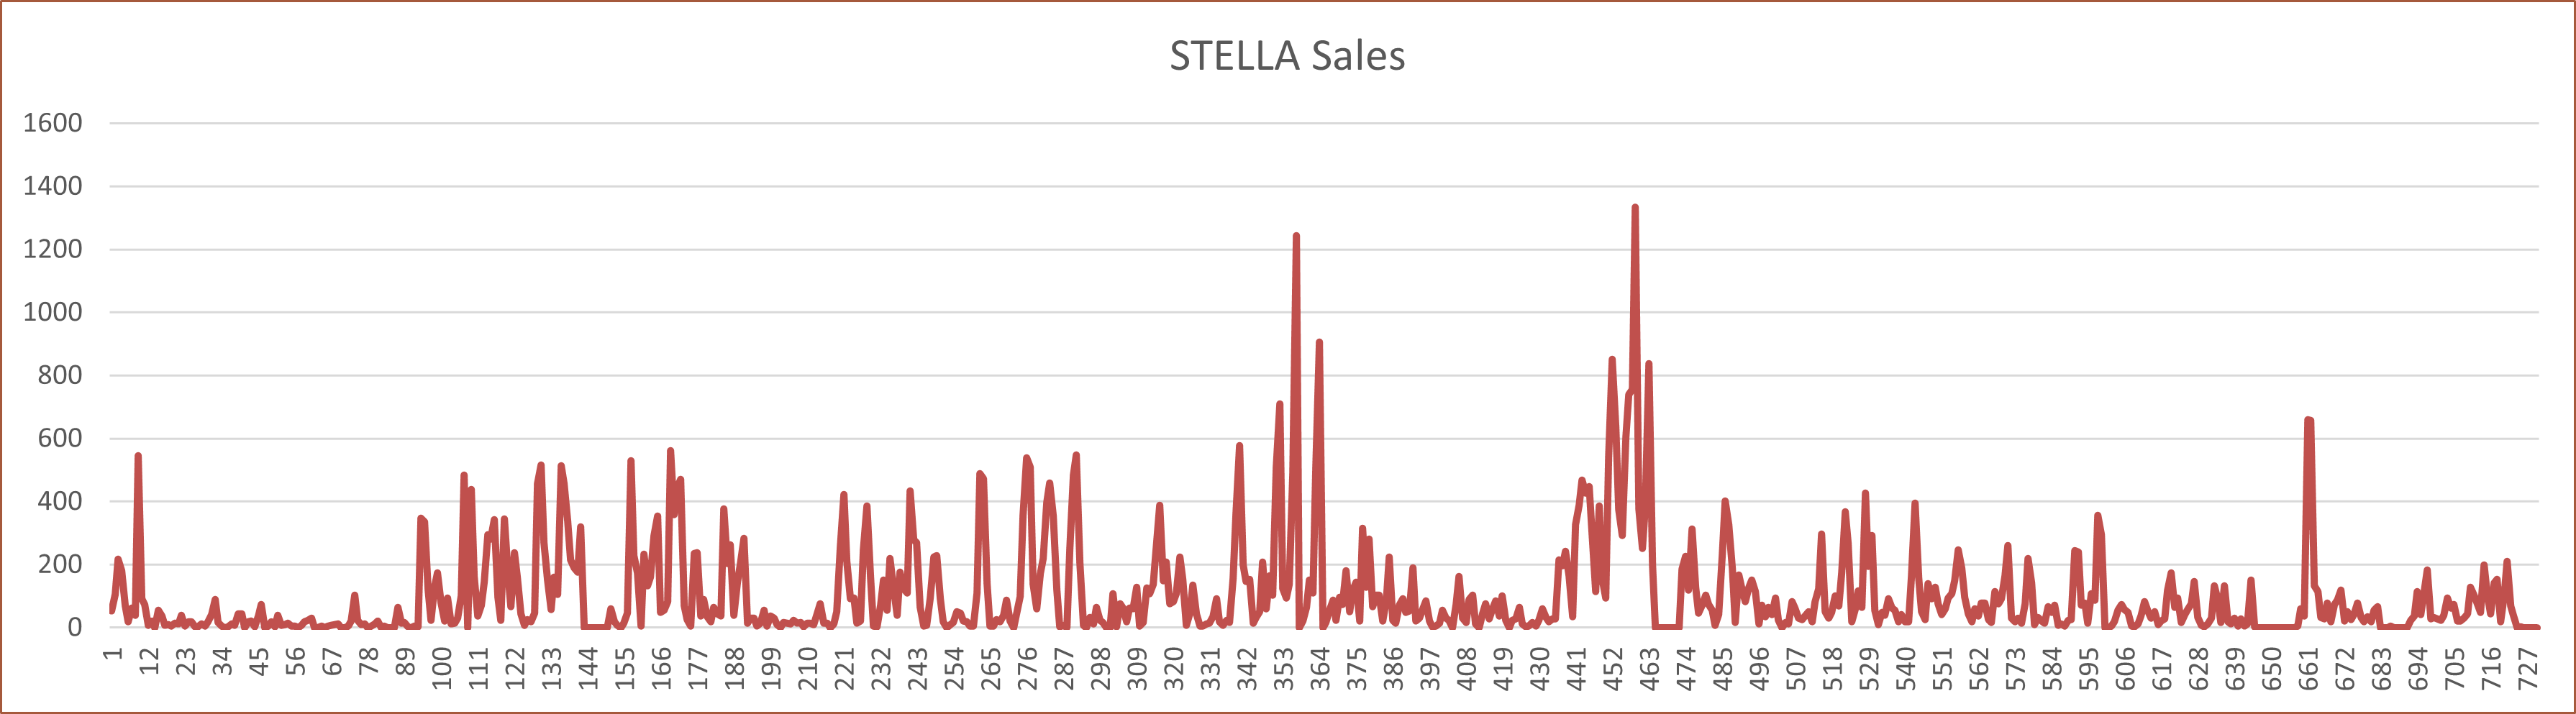
\includegraphics[width=0.8\textwidth]{assets/stella.png}
    \caption{STELLA Sales}
    \label{fig:stella_sales}
    \end{figure}

